% CVPR 2022 Paper Template
% based on the CVPR template provided by Ming-Ming Cheng (https://github.com/MCG-NKU/CVPR_Template)
% modified and extended by Stefan Roth (stefan.roth@NOSPAMtu-darmstadt.de)

\documentclass[10pt,twocolumn,letterpaper]{article}

%%%%%%%%% PAPER TYPE  - PLEASE UPDATE FOR FINAL VERSION
%\usepackage[review]{cvpr}      % To produce the REVIEW version
%\usepackage{cvpr}              % To produce the CAMERA-READY version
%\usepackage[pagenumbers]{cvpr} % To force page numbers, e.g. for an arXiv version

% Include other packages here, before hyperref.
\usepackage{graphicx}
\usepackage{amsmath}
\usepackage{amssymb}
\usepackage{booktabs}
\usepackage[export]{adjustbox}
\graphicspath{{./Images/}}

% It is strongly recommended to use hyperref, especially for the review version.
% hyperref with option pagebackref eases the reviewers' job.
% Please disable hyperref *only* if you encounter grave issues, e.g. with the
% file validation for the camera-ready version.
%
% If you comment hyperref and then uncomment it, you should delete
% ReviewTempalte.aux before re-running LaTeX.
% (Or just hit 'q' on the first LaTeX run, let it finish, and you
%  should be clear).
\usepackage[pagebackref,breaklinks,colorlinks]{hyperref}


% Support for easy cross-referencing
\usepackage[capitalize]{cleveref}
\crefname{section}{Sec.}{Secs.}
\Crefname{section}{Section}{Sections}
\Crefname{table}{Table}{Tables}
\crefname{table}{Tab.}{Tabs.}


%%%%%%%%% PAPER ID  - PLEASE UPDATE
\def\cvprPaperID{*****} % *** Enter the CVPR Paper ID here
\def\confName{CVPR}
\def\confYear{2022}

\begin{document}

%%%%%%%%% TITLE - PLEASE UPDATE
\title{BREAST CANCER DETECTION USING DIFFERENT CLASSIFIER MODELS}

\author{Botchway Kodjo Opoku\\
Oklahoma State University\\
Stillwater, OK\\
A20338464\\
{\tt\small botchwaykodjo@gmail.com}}
% For a paper whose authors are all at the same institution,
% omit the following lines up until the closing ``}''.
% Additional authors and addresses can be added with ``\and'',
% just like the second author.
% To save space, use either the email address or home page, not both
\maketitle

%%%%%%%%% ABSTRACT
\begin{abstract}
   Breast cancer is a disease that stems from the uncontrollable increase in the cells situated in the breast region. This cancer occurs most frequently in women and very rarely in men, accounting for a large percentage of cancers affecting people today. Most of the constitutions of breast cancer patients happen to be women, and even though a lot of awareness is being created to shed light on it, there is still so much to be done to increase proactivity. The early detection of abnormally growing or maturing cells is a critical step forward in the treatment process to enable doctors and physicians to save time, reduce the severity, and in extreme cases, prevent fatal endings. This paper builds a classification model for different breast cancer cell samples. The plan for approaching the problem is to categorize and correctly predict the diagnosis of breast cancer data, whether they are malignant or benign. To do this efficiently to the highest degree, we would use different traditional machine learning algorithms and a multilayer neural network to develop models and generate comparisons amongst them through hyperparameter tuning and alterations. Our model's accuracy will help detect cancer cells in patients with the recorded data. The initial results at this stage show that the classifier model, given the dataset's features, does an excellent job in classifying the cells and would help, being used hand in hand with actual experts to help deduce the probability of a patient having breast cancer.
\end{abstract}

%%%%%%%%% BODY TEXT
\section{Introduction}
\label{sec:intro}

Breast cancer is a type of cancer that originates in the breast tissue. It is the second most common type of cancer in women, and it can also affect men, although this is much less common.  The disease exists at such a heterogeneous level that targeting particular cells in an attempt at remedy is seemingly impossible. There are also different types of breast cancer and other effects on the human body. These are dependent on which cells mutate into cancerous cells. (Breast Cancer, 2022) The methods and approaches for therapy have changed over the past decades to accommodate this heterogeneity, with more attention and focus directed towards more biologically targeted medicines and treatment de-escalation to lessen side effects. 
There are several reasons why it is important to get tested for breast cancer. First and foremost, early detection of breast cancer can greatly improve the chances of successful treatment. When breast cancer is detected at an early stage, it is often smaller and has not yet spread to other parts of the body. This means that treatment can be more effective and less invasive.
Additionally, getting tested for breast cancer can help to identify any potential problems before they become more serious. For example, mammograms (a type of breast cancer test) can detect lumps or abnormalities in the breast tissue that may be early signs of cancer. By identifying these abnormalities early, doctors can take steps to monitor and treat them before they develop into cancer.
Early breast cancer is also considered treatable if confined within the breast or has only progressed to the auxiliary lymph nodes. Improvements in multimodal therapy have increased the likelihood that 70–80\% of patients will recover. \cite{Harbeck}

Even with this, in retrospect, many people still suffer from the fatality of breast cancer. In many cases, the patients or those affected are either unaware of it or do not get diagnosed when the cancer is in its early stages. This is not specific to those with an idea or a lead that nudges them to get tested but to everyone, especially women, to get checks now and then.
%-------------------------------------------------------------------------
\subsection{Problem Statement}

The main idea of this project is to use the data from the digitized images of a breast mass to make accurate deployable classifications of the samples to detect breast cancer. The dataset that will be used for the project is obtained from \href{http://archive.ics.uci.edu/ml/datasets/Breast+Cancer+Wisconsin+\%28Diagnostic\%29}{Breast Cancer Dataset}. To effectively accomplish this, we will use different machine learning models and weigh and compare the accuracy of the resulting models. Using the features provided in the dataset, the plan is to use three traditional ML classifier models, a multi-layer feed-forward neural network model, and a simple CNN model. The reason for testing these different models is to obtain the model with the highest classification accuracy. We plan to use different hyperparameters to optimize the models and ensure that the model's complexity and efficiency are not compromised.

\subsection{Background Preamble}

Some work has been done on the detection based on the actual images from patients. This will be the baseline to understand whether the results are positive. This is not particularly necessary for this project, but we wanted some domain knowledge to weigh our results against real-life instances. The results are going to be evaluated both qualitatively and quantitatively for context. Plots will also be made between the predicted and actual values. We will use different binary evaluation measures for calculating our model performance, including R-square value, misclassification score, precision, and the F1 score.

%------------------------------------------------------------------------
\section{Background/Related Work}
\label{sec:literature review}

Research classifying the cells in potential breast cancer patients has been ongoing for quite some time. This section identifies the relevant background work related to the project. Much of the available information being collected and improved involves making classifications using the actual scanned images of the tissues. Hameed and his team conducted research directed toward using an ensemble of deep-learning models to classify breast cancer histopathology images. \cite{Hameed} The accuracy in classifying the actual images came to about 95.29\%, and they were able to conclude that the experiment's results showed the effectiveness of the approach to solving this problem. Another deep learning approach adopted by Krigitha achieved similarly good results, with values of accuracy, sensitivity, and specificity of 0.986, 0.947, and 0.964. \cite{Krigitha}
Experiments by Y. M. George and his team also showed that the results of using the four different models, Multilayer perceptron, probabilistic neural network, learning vector quantization, and SVM showed effective and comparable results even in other circumstances. \cite{George} They also claimed that their results were better and that the model applied to multiple problems.
Most of these approaches were considered using different deep learning approaches. Other works were also tackled using conventional machine learning algorithms. In the study by TIWARI \cite{TIWARI}, the classification problem was handled additionally using logistic regression and K-Nearest Neighbour in addition to a neural network model and an SVM model. In this work, the data used for the classification was extracted from image data and not the candid images themselves, similar to the work done in this study.


%-------------------------------------------------------------------------
\section{Approach}
\label{sec:Approach}
\subsection{Data Preparation}

The data preparation section of a research paper is an essential part of the study as it describes the steps taken to collect, clean, and organize the data used in the analysis. This section provides a clear and detailed account of the data sources, preprocessing steps, and any transformations or manipulations performed on the data. As mentioned, the data was obtained from \href{http://archive.ics.uci.edu/ml/datasets/Breast+Cancer+Wisconsin+\%28Diagnostic\%29}{Breast Cancer Dataset}. There was no cleaning or manipulation required for this dataset. There was no missing data or data imputation needed in this case.
Working with the data, the next process was to build some internal understanding of the problem and get results that best represent the classification problem. To do this, we explored distributions of the model features and identified whether there was a need for any further feature engineering to be performed on the independent variables as shown in \textbf{Figure 1}.

\begin{figure}
    \centering
    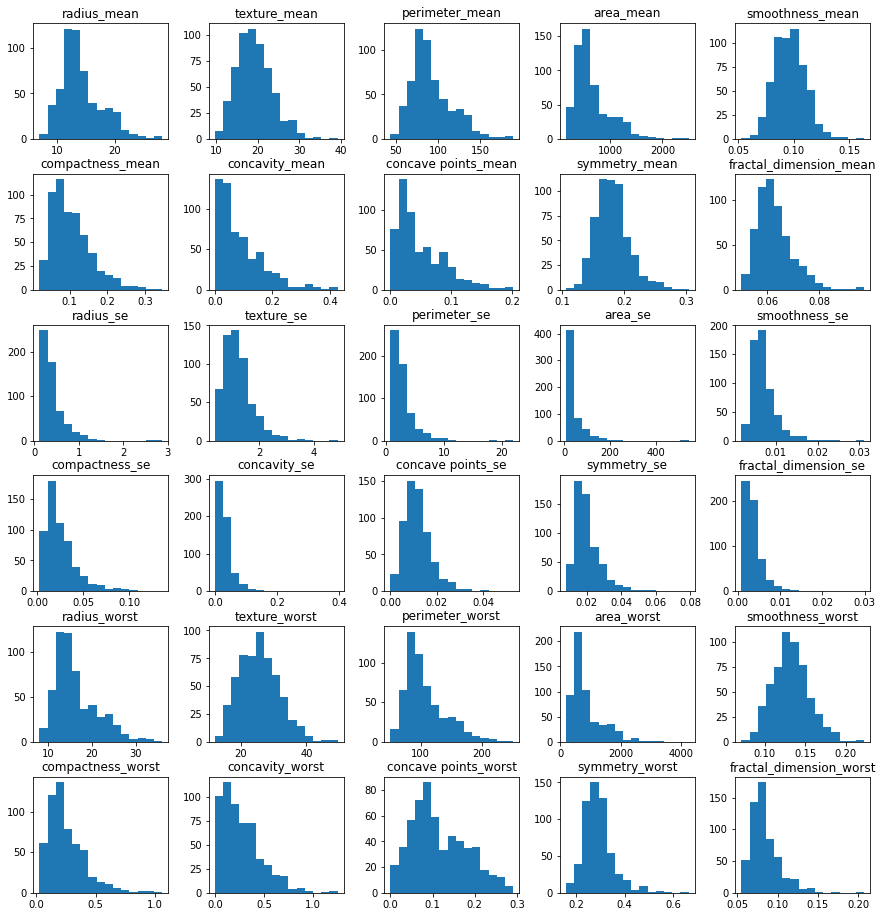
\includegraphics[width=\linewidth, height=\textheight,keepaspectratio]{Images/output.png}
    \caption{Distributions of variables in the dataset}
    \label{fig:my_label}
\end{figure}

Since the distributions of the independent variable had different spreads across the values, normalization was prudent to be performed on the data to correctly accord weightage to the independent variables. The "RobustScalar" and the "StandardScalar" sklearn packages were considered for this procedure. Still, since we did not have outliers that appeared to be influential when inserted in the machine learning algorithm, we went with StandardScalar. The target variable, 'Diagnosis,' was also explored in terms of the distribution across the different classes. (\textbf{Figure 2})

\begin{figure}
    \centering
    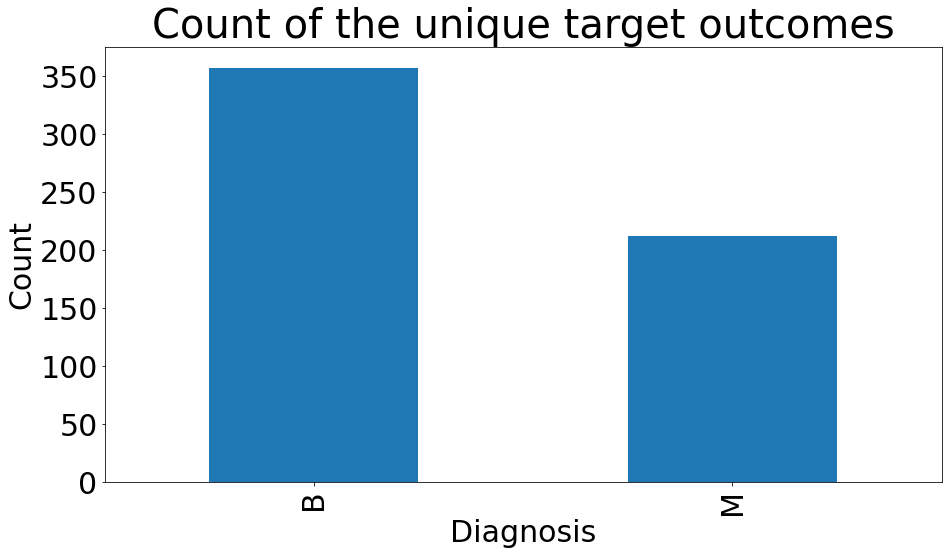
\includegraphics[width=\linewidth, height=\textheight,keepaspectratio]{Images/output1.png}
    \caption{Distribution of the classes under the target variable}
    \label{fig:my_label}
\end{figure}

Following the breakdown of the counts of the target variable, there was a raised concern about whether this would be an imbalanced dataset. Still, under further investigation and from different sources, one being \cite{Mazumder}, a dataset with a distribution of 40:60 would not exactly be considered an imbalanced dataset. With this, I went forward without balancing the data. As an added assurance my results would not be affected, I used the classification report and the confusion matrix as a benchmark for testing my solutions so that I was confident the results and interpretations were not affected and the integrity was maintained. The features of the data were then split into testing and training data to be used in the section for model deployment.

%-------------------------------------------------------------------------
\subsection{Machine Learning Algorithms}

This study employed five machine learning algorithms with a multilayer feedforward neural network model. The algorithms used at this stage were: Logistic Regression, Random Forest Classification, Decision Tree Classification, Support Vector Machines (SVM), and, as mentioned, a neural network. These were incorporated through python libraries and packages for model deployment.
Logistic Regression
Logistic regression is a simple yet powerful linear classification algorithm used to predict a binary outcome, such as whether a patient has breast cancer. It works by finding the linear decision boundary that best separates the two classes. 
Random Forest Classification
On the other hand, random forest classification is an ensemble learning method that uses multiple decision trees to make predictions. It works by training multiple decision trees on different data subsets, then averaging their predictions to get a more accurate and stable estimate. This approach is often more accurate than a single decision tree and can also be less prone to overfitting.
Decision Tree Classification
Decision tree classification is a simple and intuitive algorithm used to predict a target label based on the values of other features in the data. It works by splitting the data into smaller and smaller subsets based on the importance of each feature and then using these splits to make predictions about the target label. This can be efficient for many classification tasks, including breast cancer classification. 
Support Vector Machines
Support vector machines (SVMs) are another popular classification algorithm often used for difficult or complex classification tasks. They work by finding the decision boundary that maximally separates the two classes and can be very effective in high-dimensional data. 
Neural Network
Finally, a neural network is a machine learning algorithm composed of many interconnected processing nodes called neurons. It works by learning the relationships between the input data and the target label and then using those relationships to predict new data. Neural networks are often used for complex classification tasks, such as breast cancer classification, and can achieve very high accuracy when trained on large and representative datasets. 
These are the models that were going to be employed in this paper.

%-------------------------------------------------------------------------
\section{Code Reuse}
\label{sec:Incorporated Code}

For this project's scope, a lot of the code used was incorporated and learned throughout my degree program. Other sources of code that were included in the notebook were from the sources listed below:
\begin{enumerate}
    \item \href{https://stackoverflow.com/}{Stack Overflow} for solutions for incorrectly running code.
    \item \href{https://github.com/milaan9/93\_Python\_Data\_Analytics\_Projects/blob/main/007\_Breast\_Cancer\_Prediction\_with\_ML}{Github Help} for insights.
    \item \href{https://towardsdatascience.com/}{Towards Data Science} to understand some more information about the fundamental uses of the selected model and their interpretations.
    \item \href{https://www.w3schools.com/}{W3 Schools} for some code testing.
    \item Course material from CS 5783-65257
\end{enumerate}

Most of the code, however, was coded by me, through and through. I did seek a lot of guidance from other random google sources and random sources, but I wrote the majority of the code.

%-------------------------------------------------------------------------
\section{Experiment}
\label{sec:Results and Discussion}
\subsection{Results}

The results of running the models show that they are doing very well on the classification problem in terms of the accuracy of the training and validation sets. To ensure the accuracy values we obtained from the models, I did some k-fold cross-validations and represented the accuracy as a mean of the procedure. I used a value of 10 splits for the k-fold validation and a scoring metric based on 'accuracy.' The accuracy across the six models is greater than 90 percent. This primarily would have been good considering the raw accuracy values. \textbf{Figure 3} and \textbf{Figure 4} are depictions of these accuracies and the comparisons among each other. In the training datasets, the best-performing model was the neural network model and the lowest-performing, though still good, was the Decision Tree model.
Regarding the validation accuracies, the neural network model performed best; this time, the random forest classifier was the lowest performer. However, since the problem classification is to make sure that we can accurately classify the malignant and benign cases, we would be geared toward getting a higher specificity score, the correctly predicted malignant classes, as a ratio to the overall malignant classes. We would want this value to be as close to one as possible because the idea is to accurately predict the malignant classes of the model instead of getting a high accuracy. For example, we consider outcome one, where all malignant cases are correctly identified as malignant, and some benign cases are considered malignant with an accuracy value of 0.95. The second outcome would have most malignant identified as such and just a few malignant classed as benign with an accuracy of 0.98. For our problem statement solution, we would prefer outcome one because, even with the lower accuracy, it is doing better in grouping all the cases we should be concerned about than just getting a higher accuracy.
\begin{table}
  \centering
  \begin{tabular}{@{}lc@{}}
    \toprule
    Model & Training Accuracy \\
    \midrule
    Logistic Regression & 0.9780 \\
    Decision Tree & 0.9363 \\
    Random Forest & 0.9516 \\
    SVM & 0.9779 \\
    MultiLayer & 0.9912 \\
    \bottomrule
  \end{tabular}
  \caption{Training Accuracy}
  \label{tab:example}
\end{table}

\begin{figure}
    \centering
    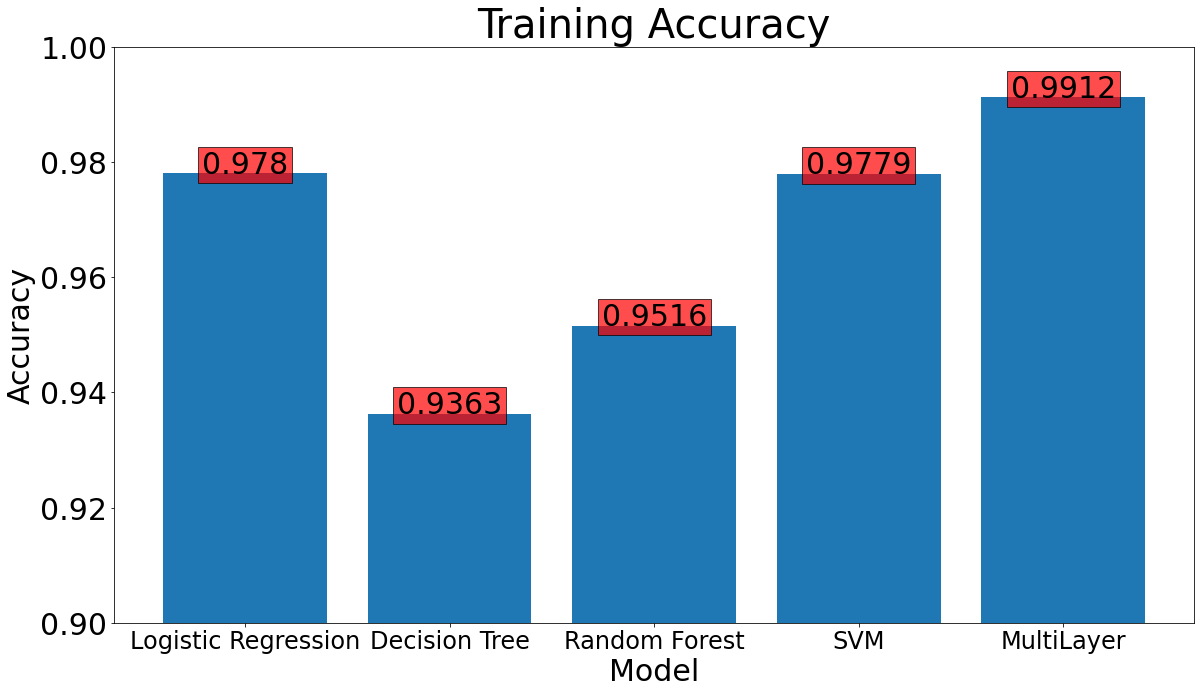
\includegraphics[width=\linewidth, height=\textheight,keepaspectratio]{Images/output2.png}
    \caption{Training accuracy values of the models}
    \label{fig:my_label}
\end{figure}

\begin{table}
  \centering
  \begin{tabular}{@{}lc@{}}
    \toprule
    Model & Validation Accuracy \\
    \midrule
    Logistic Regression & 0.9737 \\
    Decision Tree & 0.9474 \\
    Random Forest & 0.9561 \\
    SVM & 0.9737 \\
    MultiLayer & 0.9737 \\
    \bottomrule
  \end{tabular}
  \caption{Validation Accuracy}
  \label{tab:example}
\end{table}

\begin{figure}
    \centering
    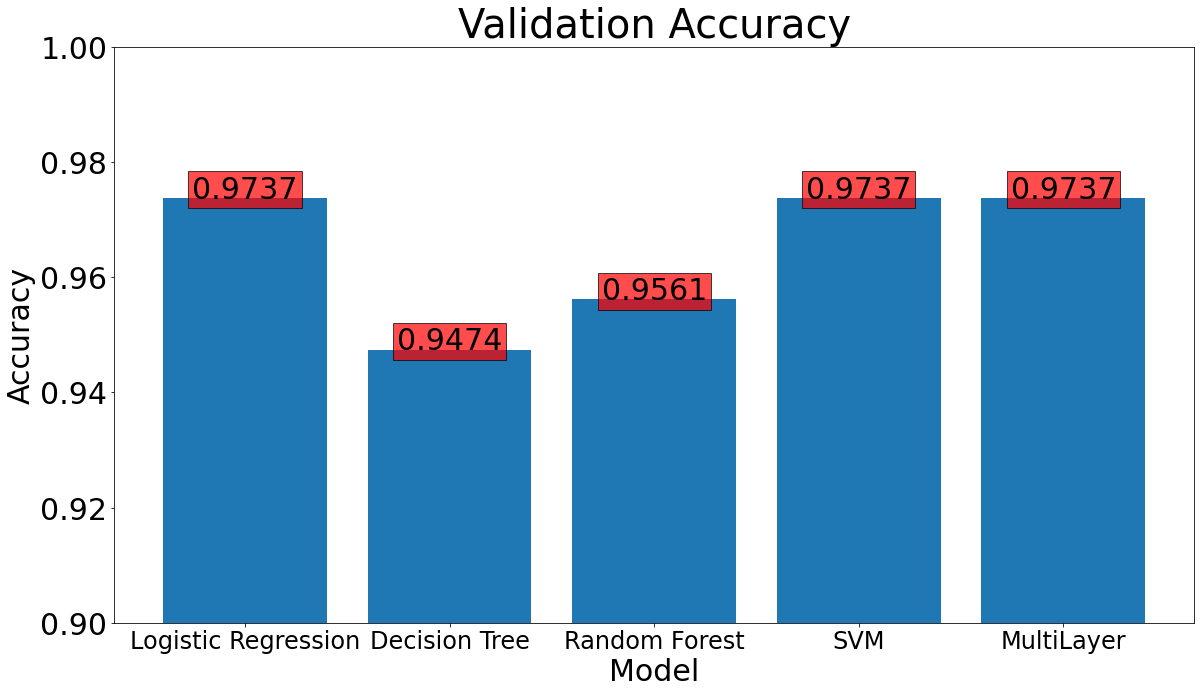
\includegraphics[width=\linewidth, height=\textheight,keepaspectratio]{Images/output3.png}
    \caption{Validation accuracy values of the models}
    \label{fig:my_label}
\end{figure}

%-------------------------------------------------------------------------
\subsection{Discussion}

For the interpretation of the results from the experiment, I decided to go into further detail in evaluating the model based on the information provided in the confusion matrix. As explained before, I was more focused on the false negative classifications before the accuracy values for this project's scope. Again, this is because, in a scope such as this, it would not be an issue if a benign breast cancer case was mistaken for a malignant one. Here, it would mean the patients will be subject to further tests and screenings even though it was probably unnecessary. That is acceptable. However, we would not want a malignant case to be classified as benign because that would be overlooked and potentially harmful and fatal to the patient. Considering this, we used the recall values for all the models for the first evaluation of the best model to use.

\begin{figure}[!ht]
    \centering
    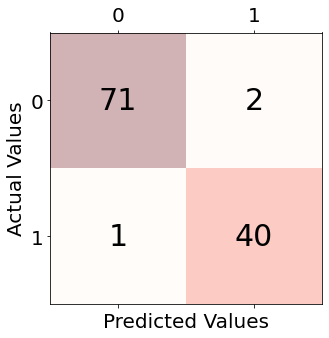
\includegraphics[width=5cm, height=5cm, keepaspectratio]{Images/output4.png}
    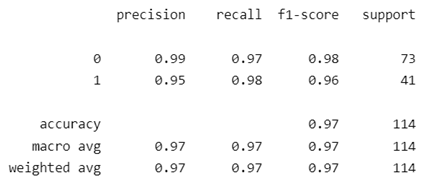
\includegraphics[width=5cm, height=5cm, keepaspectratio]{Images/Picture6.png}
    \caption{Confusion Matrix and Accuracy values for Logistic Regression}
    \label{fig:my_label}
\end{figure}

\begin{figure}[!ht]
    \centering
    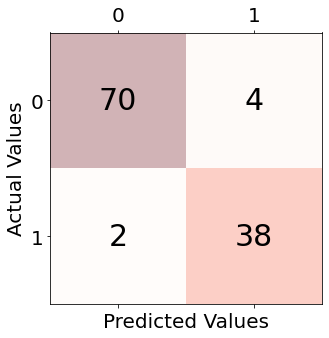
\includegraphics[width=5cm, height=5cm, keepaspectratio]{Images/output5.png}
    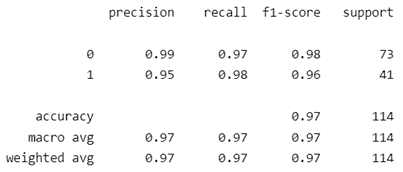
\includegraphics[width=5cm, height=5cm, keepaspectratio]{Images/Picture8.png}
    \caption{Confusion Matrix and Accuracy values for Decision Tree}
    \label{fig:my_label}
\end{figure}

\begin{figure}[!ht]
    \centering
    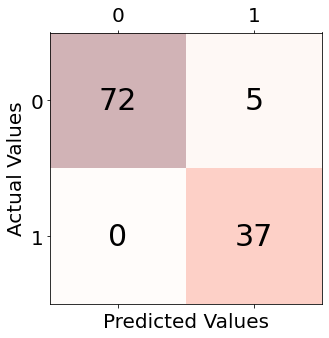
\includegraphics[width=5cm, height=5cm, keepaspectratio]{Images/output6.png}
    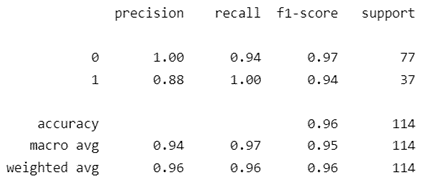
\includegraphics[width=5cm, height=5cm, keepaspectratio]{Images/Picture10.png}
    \caption{Confusion Matrix and Accuracy values for Random Forest}
    \label{fig:my_label}
\end{figure}

\begin{figure}[!ht]
    \centering
    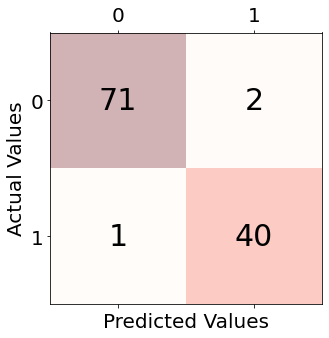
\includegraphics[width=5cm, height=5cm, keepaspectratio]{Images/output7.png}
    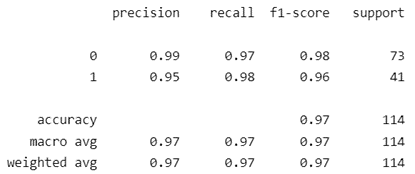
\includegraphics[width=5cm, height=5cm, keepaspectratio]{Images/Picture12.png}
    \caption{Confusion Matrix and Accuracy values for SVM Classifier}
    \label{fig:my_label}
\end{figure}

\begin{figure}[!ht]
    \centering
    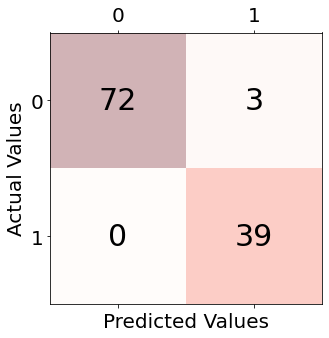
\includegraphics[width=5cm, height=5cm, keepaspectratio]{Images/output8.png}
    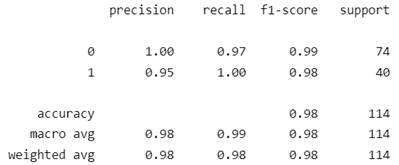
\includegraphics[width=5cm, height=5cm, keepaspectratio]{Images/Picture14.png}
    \caption{Confusion Matrix and Accuracy values for Neural Net Model}
    \label{fig:my_label}
\end{figure}

The results eventually directed towards the neural network model and the random forest models having the highest recall score for the malignant cases. This was the initial evaluation. Since we had more than one model with a recall score of 1, I decided to go with the model with the highest accuracy between the two chosen ones. That ended up being the Multilayer Feedforward Neural Network model. See the figures shown in \textbf{Figure 5 - 9} for the illustration.

%-------------------------------------------------------------------------
\section{Conclusion}

After experiments with multiple machine learning models, it was found that a neural network model outperformed all other models in terms of accuracy and recall for breast cancer classification. The neural network demonstrated a high-performance level and effectively accurately classified breast cancer cases. This suggests that neural networks may be a promising approach for breast cancer classification in the future. As a future project scope, I would want to explore different tuning of the hyperparameters in the machine learning model to determine if changing some of the default variables would lead to better accuracy metric values.

%------------------------------------------------------------------------
\section{Division of Labor}

I completed the project scope and the work done for this paper, so there is no division of labor.

%%%%%%%%% REFERENCES
{\small
\bibliographystyle{ieee_fullname}
\bibliography{egbib}
}

\end{document}
